% !TEX root = marvin.tex
\begin{figure*}[t]
\centering
\iflatexml
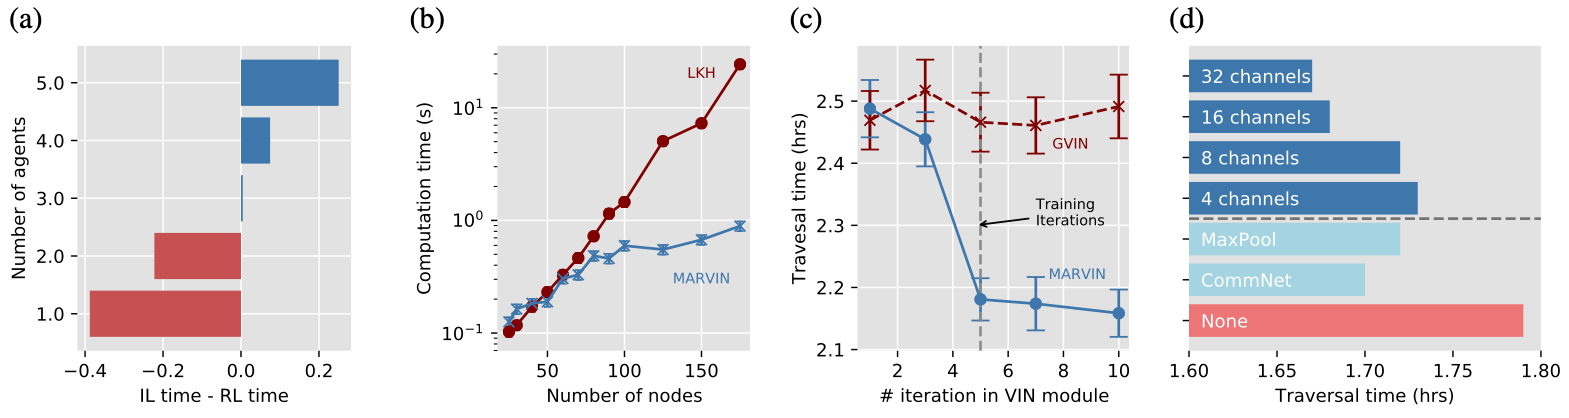
\includegraphics[width=6\textwidth]{figs/figall.png}
\else
\begin{small}
\vspace{-0.1in}
\begin{tabular}{llll}
(a) & (b) & (c) & (d)\\
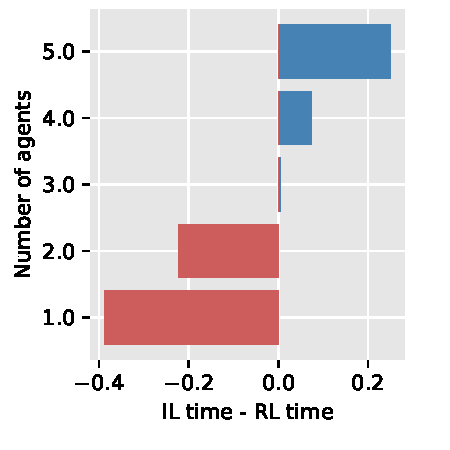
\includegraphics[height=4.1cm,trim={0.2cm 0 0.4cm 0},clip]{figs/diff_cost.pdf} &
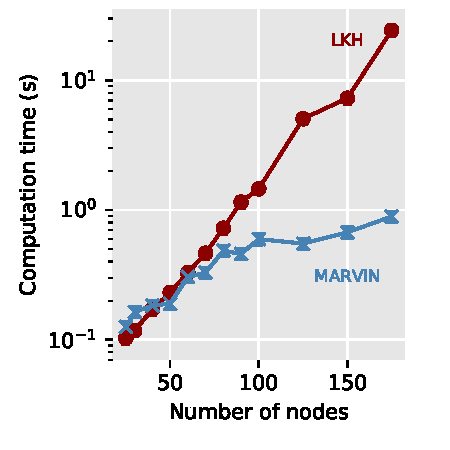
\includegraphics[height=4.1cm,trim={0.2cm 0 0.8cm 0},clip]{figs/runtime.pdf} &
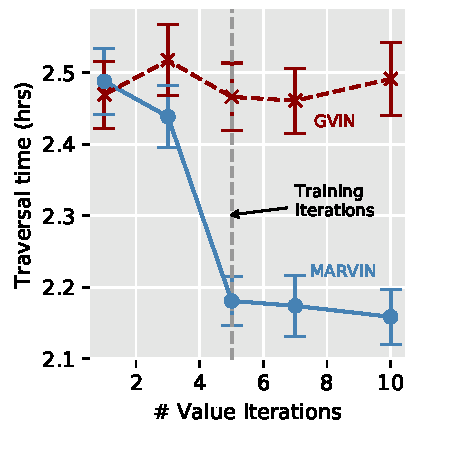
\includegraphics[height=4.1cm,trim={0.2cm 0 0.8cm 0},clip]{figs/iterations} &
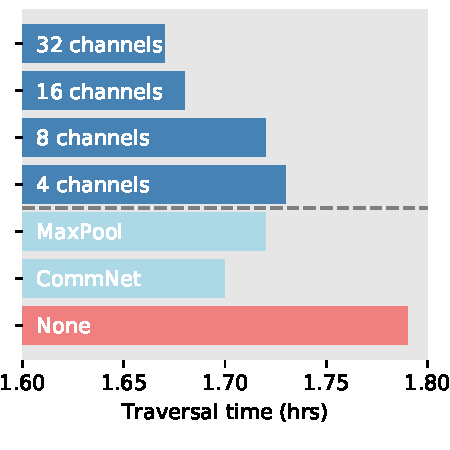
\includegraphics[height=4.1cm,trim={0.0cm 0 0cm 0},clip]{figs/comms}\\
\end{tabular}
\end{small}
\fi
\vspace{-0.1in}
\caption{\textbf{(a) IL vs. RL:} Comparison of imitation learning and reinforcement learning on different number of agents;
\textbf{(b) Runtime:} Comparison MARVIN's runtime to that of the LKH solver;
\textbf{(c) No. iterations in the VIN module:} Evaluation of how the number of value iterations has on performance, and how the number of
    iterations generally scales for other value iteration models (GVIN);
\textbf{(d) Communication module design:} Comparison of our communication protocol to other communication protocol alternatives.
}
\label{fig:all}
\end{figure*}